%%%%%%%%%%%%%%%%%%%%%%%%%%%%%%%%%%%%%%%%%%%%%%%%%%%%
%Dissertation template for the MSc in Statistics at the University of Sheffield
%You should not change anything between lines 4 and 39 of this file, except 
% to enter your title on line 9 and your name on line 10.
\documentclass{somasmsc}
\begin{document}
%%%%%%%%%%%%%%%%%%%%%%%%%%%%%%%%%%%%%%%%%%%%%%%%%%%%
%%%% Edit the next two lines in the obvious way %%%%
\newcommand{\yourtitle}{Your title goes here}
\newcommand{\yourname}{Your name goes here}
%%%%%%%%%%%%%%%%%%%%%%%%%%%%%%%%%%%%%%%%%%%%%%%%%%%%

%%%%%%%%%%%%%%%%%%%%%%%%%%%%%%%%%%%%%%%%%%%%%%%%%%%%
% To add your acknowledgements and abstract
% edit (and save) the files called acknowledgements.tex and
% abstract.tex (in the current directory) and
% then compose this file using pdflatex
%%%%%%%%%%%%%%%%%%%%%%%%%%%%%%%%%%%%%%%%%%%%%%%%%%%%%%%%%%
% Do not edit this file under any circumstances.
%%%%%%%%%%%%%%%%%%%%%%%%%%%%%%%%%%%%%%%%%%%%%%%%%%%%%%%%%%

\title{\yourtitle}

\author{\yourname
\\$~$\vspace{0.5in}\\
School of Mathematics and Statistics\\
University of Sheffield}

\date{$~$\vspace{1.5in}\\

\includegraphics[width=4in]{logo.jpg}\\
\vfill Dissertation submitted as part of the requirements for the award of MSc in Statistics, University of Sheffield, 2021--2022\\
}

\pagestyle{empty}
\frontmatter
\maketitle
\pagestyle{plain}
\tableofcontents
\newpage

\chapter{Acknowledgements} 
\setcounter{page}{1}
I would like to thank ...
\chapter{Lay Summary of the Dissertation}

Please provide here a summary of your dissertation aimed at a lay reader i.e.\ someone with a good general education, but no university level training in mathematics or statistics.   It should summarise the content, method and results and be one to two pages in length. If in doubt about the content or style of this chapter, please consult your Dissertation Support Worker.

%setup some simple running headers
\setlength{\headheight}{16pt}
\fancyhead{}
\fancyfoot{}
\pagestyle{fancy}
\fancyhead[RO,LE]{\thepage}
\fancyhead[LO,RE]{\rightmark}

%setup commenting
\newcommand{\studentcomment}[1]{\todo[inline, backgroundcolor=blue!30]{\textsc{\yourname:} #1}}
\newcommand{\DSWcomment}[1]{\todo[inline, backgroundcolor=green!30]{\textsc{DSW:} #1}}
\newcommand{\supcomment}[1]{\todo[inline, backgroundcolor=red!30]{\textsc{Supervisor:} #1}}

\mainmatter

%%%%%%%%%%%%%%%%%%%%%%%%%%%%%%%%%%%%%%%%%%%%%%%%%%%%
%%%%%%%%%%%%%%%%%%%%%%%%%%%%%%%%%%%%%%%%%%%%%%%%%%%%

%%%%%%%%%%%%%%%%%%%%%%%%%%%%%%%%%%%%%%%%%%%%%%%%%%%%
% You should write the main part of your thesis below here
%%%%%%%%%%%%%%%%%%%%%%%%%%%%%%%%%%%%%%%%%%%%%%%%%%%%

\chapter{Introduction}\label{intro}
You can call your first chapter (and all the others) whatever you wish, but it is usual to start with an introduction to your project and, perhaps, a discussion of some background literature.

When you are discussing other people's work, you might find the following snippets of \LaTeX\ helpful.  You might make references like these if you want to discuss the work of \citet{lambert} and \citet{dellas} within a sentence. Then, later, you might also want to make some parenthetic references to support an argument that you are making, like this \citep{lambert}.  Alternatively, we might want to say that in \citeyear{lambert} a key paper was published by \citeauthor{lambert} in which they demonstrated that ...

In the next chapter, we provide some more snippets that you might find useful.  We do not give advice about the structure of the dissertation here, since that is covered in the separate document on Dissertation Expectations (on Blackboard), but do remember the very strict page limit of 70 pages in the \verb+\mainmatter+ of your dissertation. Those working on theoretical topics, with little need for figures and tables in their dissertation, should aim for considerably fewer than 70 pages (typically 30--50).  If you do submit something longer, examiners will read only the first 70 pages (or 50  pages of more theoretical material).  Note too that, regardless of length, any material in appendices will only be inspected cursorily by examiners. You should thus use appendices judiciously.


\chapter{Some reminders}\label{reminders}

For all the basics of typesetting, that you are likely to need in your dissertation, please use the handouts on \LaTeX\ that you were given earlier in the MSc or consult or the single document on \LaTeX\ provided on the dissertation Blackboard page.  Below we provide further snippets of code, inspired by the Wikipedia entry on L\'{e}vy's continuity theorem, to remind you of some key typesetting concepts that you should be aware of.

Before we do that, however, just a quick note on editing and commenting on your writing. First, you might find the online \LaTeX\ editor called Overleaf helpful for working on your dissertation and sharing it with your Support Worker. Instructions for using Overleaf in this way are provided on Blackboard. Second, note that we have defined some extra \LaTeX\ commands within this template to help when discussing your writing with others. You are not required to use these commands, but we hope that you (and the staff working with you) might find them useful.
\supcomment{This is a comment on the student's work by the supervisor.}
\DSWcomment{This is a comment on the student's work by the DSW.}
\studentcomment{This is a query related to the above comment.}

\section{A key theorem}\label{theorem}

Later we will find it useful to remember L\'{e}vy's continuity theorem (Theorem~\ref{theorem:levyct}), which we do not prove since it is fairly well known, but complete proofs are available in \citet[section 18.1]{Williams} and \citet[Theorems 14.15 and 18.21]{Fristedt}.


\begin{theorem}\label{theorem:levyct}
 Suppose we have
\begin{itemize}
\item a sequence of random variables $\{X_n\}_{n=1}^\infty$, not necessarily sharing a common probability space,
\item the sequence of corresponding characteristic functions $\{\varphi_n\}_{n=1}^\infty$, which by definition are:
$$
\varphi_n(t) = \E e^{itX_n} \quad \forall t\in\mathbb{R},\ \forall n\in\mathbb{N},
$$
where $\E$ is the expected value operator.
\end{itemize}
If the sequence of characteristic functions converges pointwise to some function~$\varphi$ where
$$\varphi_n(t)\to\varphi(t) \quad \forall t\in\mathbb{R},$$
then the following statements become equivalent:
\begin{itemize}
\item $X_n$ converges in distribution to some random variable $X$:
$$X_n\ \xrightarrow{\mathcal D}\ X,$$
i.e.\ the cumulative distribution functions corresponding to random variables converge at every continuity point of the c.d.f.\ of $X$;
\item $\{X_n\}_{n=1}^\infty$is tight:
$$\lim_{x\to\infty}\left( \sup_n \Prob\big[\, |X_n|>x \,\big]\right) = 0;$$
\item $\varphi(t)$ is a characteristic function of some random variable $X$;
\item $\varphi(t)$ is a continuous function of $t$;
\item $\varphi(t)$ is continuous at $t=0$.
\end{itemize}
\end{theorem}

\section{Another section}

It is often useful to refer the reader to a figure, such as Figure~\ref{Fig:Rwalk}, and you could use a similar \verb+\label+ and \verb+\ref+ technique for refering to chapters (such as Chapter~\ref{intro}), sections (such as Section~\ref{theorem}), Appendices (like Appendices~\ref{apx:prob}, \ref{apx:proofs} and \ref{apx:ethics}), as well as for tables.
\begin{figure}
\begin{center}
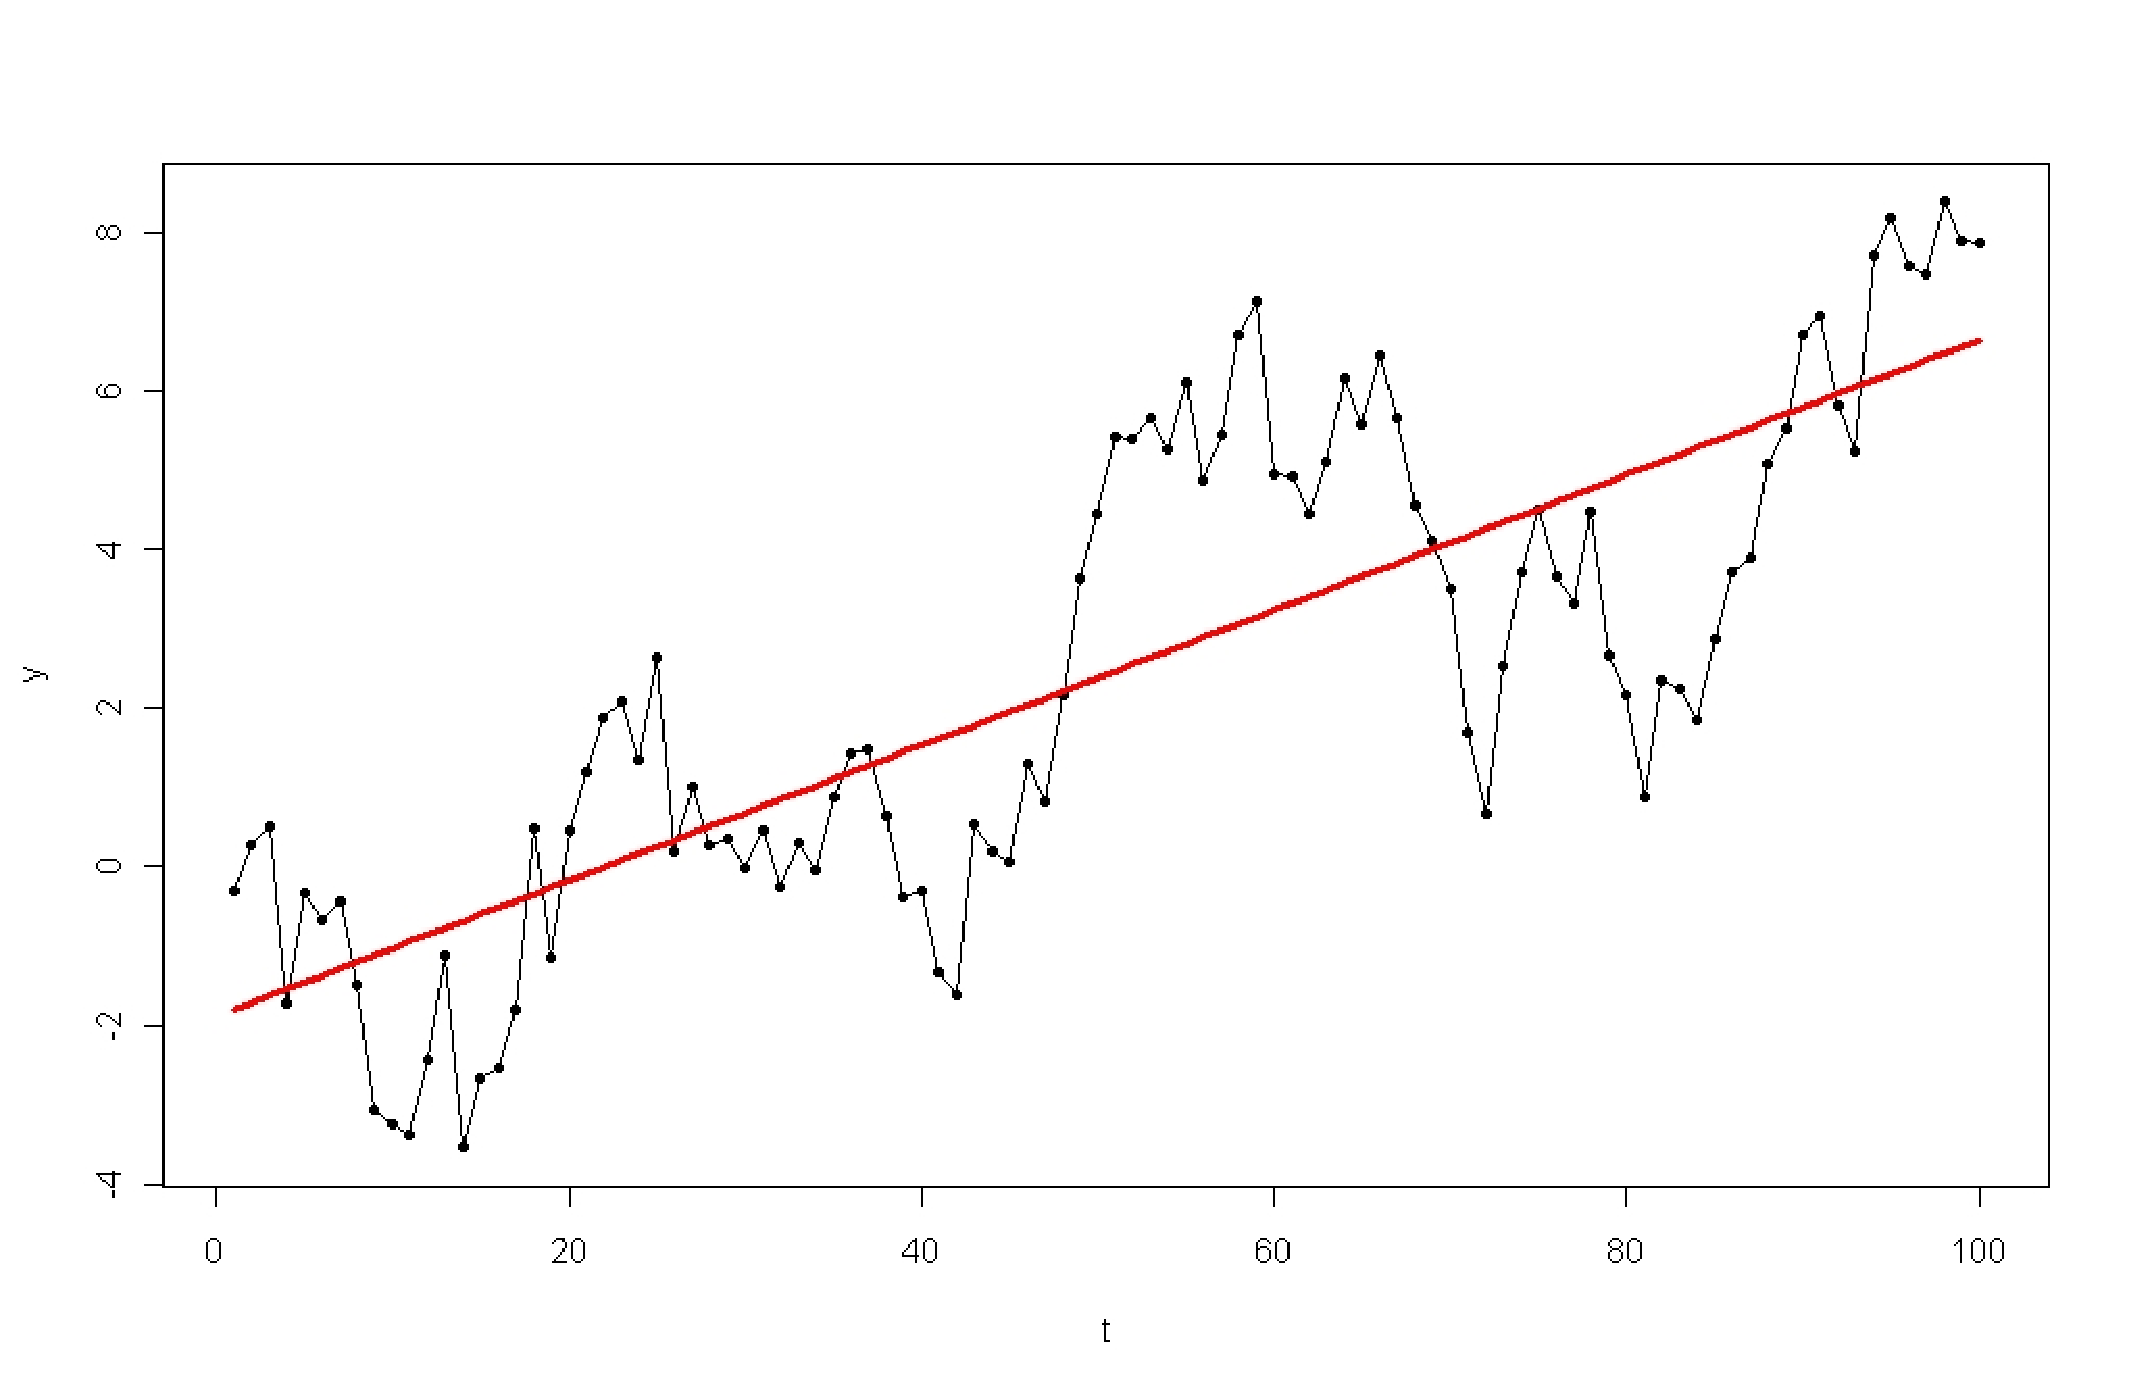
\includegraphics[width=12cm]{Rwalk.pdf}
\end{center}
\caption{Here is a horrible figure.  Note the variable names in the axis labels and the rather small tick mark labels. You must not make these mistakes in the plots for your own dissertation. Remember too the Caption Test from the EDA with R lecture notes.}
\label{Fig:Rwalk}
\end{figure}

% To amend the appendices, edit (and save) the file
% in the current directory called appendices.tex and
% then recompile this file using pdflatex.


\appendix

\chapter{Review of probability calculus}\label{apx:prob}

Use appendicies only for material that is directly relevant to the contents of your dissertation and is referenced from within it.  Never use it for code or for things that you found interesting, but did not in the end use for your own work.  If you and your supervisor agree that providing examiners with code is essential then please deposit it online (via a service such as GitHub).

\section{Functions of random variables}
\section{Schwarz Inequality}

%%%%%%%%%%%%%%%%%%%%%%%%%%%%%%%%%%%%%%%%%%%%%%%%%%%%

\chapter{Some technical proofs}\label{apx:proofs}

\section{Proof 1}

%%%%%%%%%%%%%%%%%%%%%%%%%%%%%%%%%%%%%%%%%%%%%%%%%%%%

\chapter{Research Ethics Approval}\label{apx:ethics}

The last appendix of the dissertation must contain evidence that you complied with the University of Sheffield research ethics approval process. Like all other appendices, it should be cross-referenced from the main text of the dissertation so that readers are alerted to its presence. The appendix should start with a paragraph of text, in your own words, that summarises the approval process as it applied to your dissertation. Here is an example to get you started.

The research ethics approval process for the work described in this dissertation was completed in March 2019, before any work using data commenced. Due to the use of data arising from <summarise the data collection process here>, formal research ethics approval was deemed to be necessary and, when submitted, the application was allocated reference number: 000094. Formal approval is evidenced here by inclusion of the final approval letter in Figure~\ref{ethicsapprov}. 

\begin{figure}

\includegraphics[width=15cm,clip, trim=1cm 15cm 1cm 1cm]{ApprovalLetter.pdf}
\caption{The research ethics approval letter provided for the work outlined in this dissertation, following compliance with the University of Sheffield offical research ethics processes.}
\label{ethicsapprov}
\end{figure}


%%%%%%%%%%%%%%%%%%%%%%%%%%%%%%%%%%%%%%%%%%%%%%%%%%%%
% To add to or change the References, edit (and save)
% the file called references.tex in the current
% directory and then recompile this file using pdflatex.
%If the file compiles but leaves a question mark where
%you expect to see a reference, recompile using bibtex
%and then recompile using pdflatex again.
% Do not change any code below here.
%%%%%%%%%%%%%%%%%%%%%%%%%%%%%%%%%%%%%%%%%%%%%%%%%%%%

\backmatter
\renewcommand{\bibname}{References}
\bibliography{references}
\bibliographystyle{apalike}

%%%%%%%%%%%%%%%%%%%%%%%%%%%%%%%%%%%%%%%%%%%%%%%%%%%%
%%%%%%%%%%%%%%%%%%%%%%%%%%%%%%%%%%%%%%%%%%%%%%%%%%%%

\end{document}
